\chapter{Estado del Arte}\label{chapter:state-of-the-art}
Una epidemia es la aparición en un período de tiempo corto de una enfermedad infecciosa en
una población. Cuando la enfermedad persiste en la población después de un tiempo determinado, 
se considera endemia. Para los casos en que la enfermedad abarca no solo períodos de
tiempo largos, sino que además está difundida por una región geográfica grande, se denomina
pandemia.\autocite{Morens2004}
\section{Redes complejas}
En el contexto de la teoría de redes, una red compleja se refiere a una red (grafo) que posee
ciertas características topológicas no triviales que no ocurren en redes simples.\\
Newman en \autocite{Newman2003} especifica los conceptos y propiedades de estas,
en el cual expresan que las redes complejas son estructuras compuestas por un conjunto de elementos interconectados, 
donde las interacciones entre esos elementos generan propiedades emergentes a nivel global.\\ 
\\
\textbf{Propiedades de las redes complejas:} 
\begin{enumerate}
    \item Distribución de grado libre: Las redes complejas tienden a tener una distribución de grado 
    libre, lo que significa que el número de conexiones que tienen los nodos sigue una ley de potencia. 
    Esto implica que existen pocos nodos con un grado muy alto (llamados "hubs") y muchos nodos con un 
    grado bajo. Esta propiedad refleja la heterogeneidad en la conectividad de los nodos.
    \item Mundo pequeño: Las redes complejas a menudo exhiben la propiedad del mundo pequeño, lo que 
    significa que la distancia promedio entre dos nodos elegidos al azar es relativamente corta. En 
    otras palabras, los caminos entre nodos distantes suelen ser sorprendentemente cortos. Esta propiedad 
    facilita la propagación de información o influencia rápidamente a través de la red.
    \item Clustering o agrupamiento: Las redes complejas tienden a mostrar agrupamiento o clustering significativo.
    Esto significa que los nodos tienden a formar comunidades o grupos densamente conectados entre sí. Dentro 
    de una comunidad, los nodos están más interconectados que con nodos fuera de la comunidad. El agrupamiento 
    refleja la tendencia natural de las entidades a formar subgrupos o comunidades en la vida real.
    \item Centralidad: La centralidad de un nodo en una red compleja se refiere a su importancia relativa 
    en términos de conexiones o influencia. Hay diferentes medidas de centralidad, como la centralidad de 
    grado, la centralidad de cercanía y la centralidad de intermediación. Los nodos con alta centralidad 
    suelen desempeñar un papel crucial en la estructura y la dinámica de la red.
    \item Propagación y difusión: Las redes complejas influyen en cómo se propaga la información, los 
    contagios o los flujos a través de sus conexiones. Esto tiene aplicaciones en el estudio de la propagación 
    de enfermedades, la difusión de información en las redes sociales, la viralidad de contenido en línea, 
    entre otros fenómenos.
\end{enumerate}

Los ejemplos de redes complejas son numerosos en la actualidad; el cerebro es una red de neuronas
conectadas por medio de la sinapsis, una organización es una red de personas con diversos
tipos de conexiones entre ellas, la economía mundial es una red formada por las economías
nacionales, que a su vez son redes de mercados, y éstos son redes de productores y consumidores
que interactúan, las redes de transporte público, como las redes de autobuses o trenes en una ciudad, 
se pueden modelar como redes complejas; siendo los nodos las paradas y las aristas representan las 
rutas o conexiones entre ellas.

\subsection{Redes sociales}
En el contexto de las redes sociales, los individuos o entidades son los elementos de la red, 
y las interacciones o conexiones entre ellos forman las aristas. Estas redes exhiben varias propiedades 
típicas de las redes complejas, como la distribución de grado libre, donde algunos nodos tienen 
muchos enlaces mientras que otros tienen pocos; la presencia de comunidades o grupos de nodos altamente 
interconectados; y la presencia de nodos influyentes o centrales que desempeñan un papel importante en la 
red.\autocite{Newman2003}

Este tipo de redes complejas se ha utilizado para simular la propagación de enfermedades y el control que se puede
realizar para evitar su esparcimiento de muchas maneras en la actualidad. En \autocite{Eubank2004} 
se realiza una simulación en la cual se crea una red social dividida en dos grupos, las personas y los lugares, esta red 
se puede ver como un grafo bipartito:
\begin{center}
    (Sea $p$ $\subset$ Personas y $l$ $\subset$ Localizaciones)\\
    $G(V,E)$: $p$ $\in$ $V$, 
$l$ $\in$ $E$ : si $a,b$ $\in$ $V$ , $<a,b>$ $\in$ $E$, $x = w(a,b)$  $\Rightarrow$ $a$ está en el instante de tiempo $x$ en $b$
\end{center} 
Esta manera de modelar el problema de cómo representar personas y localizaciones en las simulaciones se considera 
interesante pues muchas enfermedades se transmiten mediante la interacción con una persona infectada, actuando como un 
intermediario en el proceso de contagio. Este grafo no es dinámico, es decir, mantiene su estado inicial de nodos y aristas.
Un grafo dinámico se acercaría más al comportamiento que tienen las personas en la sociedad, ya que todos los días no nos encontramos
en el mismo lugar a la misma hora.



\section{Modelos Basados en Agentes}
La simulación basada en agentes\footnote{ABM por sus siglas en inglés} es un enfoque de modelación computacional que se utiliza para 
simular sistemas complejos, donde los agentes individuales interactúan entre sí y con su entorno. Cada agente es una entidad 
autónoma con su propio comportamiento, objetivos y reglas de interacción. El estado interno,
su percepción del entorno y las interacciones con otros agentes es lo que define la decisión o acción a realizar por
estos. \autocite{Macal2010} \\ 

\textbf{Estructura de una modelación basada en agentes:}\\
\begin{enumerate}
    \item Conjunto de agentes, sus atributos y comportamientos posibles.
    \item Conjunto de las relaciones entre agentes y los métodos de interacciones.
    \item El entorno en el que interactúan.
\end{enumerate}


En un $ABM$, se busca comprender cómo emergen los patrones y las dinámicas a nivel colectivo a partir de las interacciones 
de los agentes individuales. Según Nicholas R. Jennings en \autocite{Jennings2000} la definición de agentes está dada 
por ciertos puntos:\\
\begin{enumerate}
    \item Se encuentran situados en un entorno: reciben una instancia del estado del medio y actúan en este.
    \item Tienen propósitos específicos: poseen objetivos particulares a lograr.
    \item Autonomía: tienen control sobre sus estados internos y sobre sus propios comportamientos.
    \item Capacidad de presentar comportamientos flexibles antes la soluciones de problemas siempre siguiendo sus objetivos: necesitan ser capaces de actuar en consecuencia con lo que ocurre para cambiarlo o mantenerlo y también actuar anticipadamente para esto.
\end{enumerate}

Con este modelo es posible simular diferentes escenarios; la convivencia de animales en un medio, con el 
objetivo de observar como se modifican las poblaciones del mismo se podría simular usando agentes; en este 
caso los animales se tratarían como los agentes del modelo; también para la propagación de epidemias \autocite{Bagni2002}, 
simulacros de incendios o atentados en centros de trabajo; en ambos casos, las personas serían tratadas como los agentes 
de la simulación.

En \autocite{Bissett2021} 
además de utilizar la red social, se basan en agentes para simular. En su caso las personas son agentes que 
poseen cierto grado de infección, cierta probabilidad de transmitir, tienen cierta movilidad, pero por lo 
que se interpreta estos agentes no tienen la capacidad de decidir en un instante de tiempo que hacer exactamente, 
sino que el grafo ya esta definido  de tal forma que estos se mueven por lo que en la red indica. Pero, ¿qué 
sucedería si las personas tuvieran la posibilidad de decidir; según lo que perciben del medio, según sus sentimientos; 
qué hacer en el instante de tiempo en que se encuentran? En teoría, toda persona teniendo en cuenta el 
contexto social y su presente, tiene la capacidad de realizar o no una acción determinada, por lo cual, para la pregunta 
formulada anteriormente, se interpreta que de implementarse así, un agente se comportaría similar a una persona.\\ 
Surge otra interrogante, ¿cómo lograr que los agentes se comporten de una forma u otra según lo que perciben? Una manera 
de darle respuesta a esta pregunta es mediante Mapas Cognitivos Difusos (FCM por sus siglas en inglés) 


\section{Mapas Cognitivos Difusos}
Bart Kosko en \autocite{Bart1986}
brinda un concepto de mapa cognitivo difuso, argumenta que son digrafos en los cuales los nodos son variables,
que representan conceptos y las aristas son conexiones entre estos. Sea $G$ digrafo que representa al FCM, 
sea la arista:
\begin{center}
    $<a,b>$ $\in$ $G$ si $w(a,b)$ > $0$  ($w(a,b)$ < $0$) $\Rightarrow$ El concepto que representa el nodo $a$ influye 
    positivamente (negativamente) en el concepto que representa el nodo $b$. (Los pesos de las aristas son valores desde 
    [-1,1])  
\end{center}
\begin{figure}[htb]
    \centering
    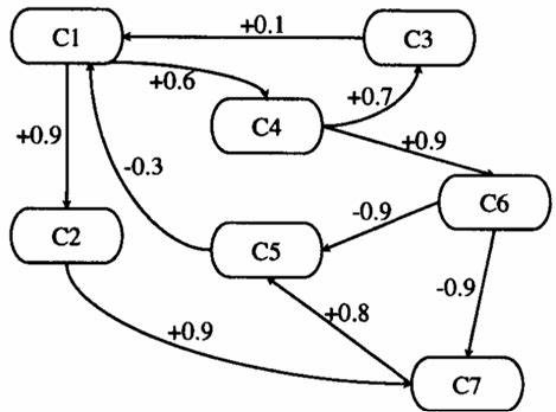
\includegraphics{Graphics/fcm_example.png}
    \caption{Ejemplo de un FCM}
\end{figure}

En esta imagen los $C_{i}$ hacen referencia al concepto $i$ del agente. El valor de los conceptos de los agentes se 
calcula en el momento en que este deba realizar una acción utilizando la siguiente función:
\begin{center}
    $X_{i}$(t+1) = F($X_{i}$(t) + $\sum_{j=1}^{n}${($X_{j}$(t) $\times$ $w_{j,i}$)})
\end{center}

donde $X_{i} (t)$ es el valor del i-ésimo concepto en el t-ésimo instante de tiempo, $i,j$=1, 2, ..., $n$, donde $n$ es el número
de conceptos, $w(i,j)$ es el peso que representa la relación que posee el concepto $i$ con el concepto $j$ y $F(x)$ es la función 
de transformación sigmoidal que normaliza los valores conceptuales al rango $[0,1]$. \autocite{Poczeta2020}

Existen varias formas y ejemplos en los cuales se puede utilizar un FCM, Nachazel en \autocite{Nachazel2021}
explica una nueva modificación a los FCM para la autonomía de decisión de los agentes. Propone dividir los conceptos en 3 clases
diferentes; necesidades, actividades y estados; para así agregar características que ayuden a la toma de decisiones y las necesidades 
internas que puede tener un agente. Es una visión sorprendente sobre en que se basa una entidad
o agente para la toma de decisiones o realizar una acción. Sin embargo, es de considerar,que utilizando otras clases, se 
puede lograr una mejor adaptación del FCM al necesitado: percepciones, sentimientos, acciones.\\ 
Con estas tres nuevas clases se podría utilizar el conocimiento que tiene un agente sobre el medio que lo rodea ($\textbf{percepciones}$) y  
cómo este se siente con respecto a esto ($\textbf{sentimientos}$) para así decidir sobre que acción final realizaría ($\textbf{acciones}$).\\

Al enlazar los conceptos y modelos antes vistos, se obtendría un entorno en el cual convivirían los agentes, teniendo o no algún
tipo de relación entre ellos (Red Social); en este existirían localidades a las cuales los mismos podrían acceder (Red Social) y 
cada agente poseería su propio FCM de percepción, sentimientos y acciones para elegir qué realizar en cada momento.